
\documentclass[titlepage]{article}
 \usepackage[utf8]{inputenc}
\usepackage{listings}
\usepackage{verbatim}
\usepackage{graphicx}
\graphicspath{ {imagenes/} }
 \usepackage{xcolor}
 \definecolor{RoyalBlue}{cmyk}{1, 0.50, 0, 0}
\usepackage{amsmath}
\lstset{language=Java,
	keywordstyle=\color{RoyalBlue},
	basicstyle=\scriptsize\ttfamily,
	commentstyle=\ttfamily\itshape\color{gray},
	stringstyle=\ttfamily,
	showstringspaces=false,
	breaklines=true,
	frameround=ffff,
	frame=single,
	rulecolor=\color{black}}


 

% Datos de la portada
\begin{document}
	\begin{titlepage}
		\begin{center}
			\vspace*{1cm}
			\date{} % para que no aparezca la fecha la dejo en blanco
			\Huge
			\textbf{Practica 2: Algoritmos Genéticos y Meméticos}
			
			\vspace{0.5cm}
			\LARGE
			Metahurística
			
			\vspace{1.5cm}
			
			\textbf{José Manuel Pérez Lendínez}
			\textbf{26051613-L}\newline
			
			\textbf{jmplz14@correo.ugr.es}		

					
			\textbf{Grupo 1 curso 18/19}
			

			
		\end{center}
	\newpage
	\tableofcontents
	\newpage
	\end{titlepage}
	\section{Descripción del problema}
	 El problema se basa en optimizar la clasificación de nuevos elementos a partir de dos particiones. La particiones de entrenamiento y la partición de test.
	 
	Tendremos un conjunto de datos que dividiremos en 5 particiones, 4 para entrenamiento y una para test. La partición de test ira rotando hasta que todas pasen por test una vez. 
	
	Los conjuntos de datos vendrán dados por una clase y un conjunto de características. Se representarán como un vector con la siguiente estructura.
	\begin{center}
		$(x_1, x_2, ... , x_n, y)$
	\end{center}

	Donde las x corresponde a las características y la y a la clase que pertenece ese elemento.
	
	El objetivo sera ser capaces de acertar con el vector de características a la clase que pertenece. Para ello entrenaremos nuestro modelo con los datos de entrenamiento y usaremos los datos de test para ver si el modelo da resultados mas o menos acertados.
	
	El clasificador tendrá que ser capaz de adivinar la clase utilizando la distancia a los datos de entrenamiento mas cercanos a la muestra elegida de los datos de test. Esta técnica se conoce como k-vecinos mas cercanos y sera la utilizada en todos nuestros algoritmos. Nosotros usaremos una k=1 por lo que solo buscaremos el vecino mas cercano para clasificar sin tener en cuenta a el mismo como vecino.
	
	Al trabajar con datos reales sera muy difícil llegar a la solución exacta por lo que se buscaran aproximaciones.
	
	Para esto utilizaremos tres metahurísticas que explicaremos a continuación y que son:
	\begin{enumerate}
		\item Algoritmo genético generacional
		\item Algoritmo genético estacionario
		\item Algoritmo memético
	\end{enumerate}
	\newpage
	
	\section{Aplicación de los algoritmos }
	 En esta parte se explicaran la representación del problema de una forma mas completa y las características comunes que tienen todos los algoritmos.
	 
	 \subsection{Descripción de la representación y calculo de distancias}
	 
	 Para representar los datos usaremos matrices de numpy para los datos, que tendrán la siguiente estructura después de cargarlos desde los fichero.
	
	\[
	datos =
	\begin{bmatrix}
	x_{1,1} & x_{1,2} & ... & x_{1,j} & y_1 \\
	. & . & . & . & . \\
	. & . & . & . & .\\
	x_{i,1} & x_{i,2} & ... & x_{i,j} & y_i
	\end{bmatrix}
	\]
	Esta matriz tendrá que ser normalizada la parte de los datos (las x) entre [0,1] para realizar con ella los cálculos de distancias para ver cual es el vecino mas cercano.
	
	Para los algoritmos RELIEF y para la búsqueda local necesitaremos un vector de pesos que se representara de la siguiente manera:
	$$
		(w_1, w_2, ..., w_j)
	$$
	Este vector sera utilizado para ponderar la importancia de las distintas características de nuestros problemas. El vector tendrá unos valores acotados entre [0,1] y tendremos en cuenta que los valores menores que 0.2 no se utilizara para calcular las distancias en la clasificación. Esto restara importancia a las variables que tengan una ponderación muy baja y que podrían introducir ruido.
	\newline
	
	En esta practica añadimos también una nueva representación a tener en cuenta para los nuevos algoritmos. Los algoritmos genéticos y meméticos costan de unas poblaciones que tendremos que almacenar para ir trabajando con estas. Cada individuo de la población sera un vector de pesos como los mencionados anteriormente. La representación de la población necesita dos características, los vectores de pesos y el valor de la función objetivo para cada individuo.
	
	Para esto usaremos una matriz para almacenar cada individuo de la población y un vector para el valor de la función objetivo para cada individuo de la población.
	
	\[
	Poblacion =
	\begin{bmatrix}
	w_{1,1} & w_{1,2} & ... & w_{1,j} \\
	. & . & . & . \\
	. & . & . & .\\
	w_{i,1} & w_{i,2} & ... & w_{i,j}
	\end{bmatrix}
	\]
	
	$$
	eval\_poblacion = (valor_1, valo_2, ..., valor_i)
	$$
	\newline
	
	
	

	
	

	
	
	\subsection{Calculo de la tasa de reducción}
	La tasa de reducción vendrá dada por la cantidad de pesos de nuestro vector w que sean inferior a 0.2 de forma que usaremos el siguiente pseudónimo para calcularla.
	La formula de la tasa de reducción es la siguiente:
	$$
		tasa_reduccion = 100 \frac{nº\ de\ w_j < 0.2}{w.size}
	$$
	El pseudocódigo seria el siguiente:
	\begin{lstlisting}
	num_reducciones = 0
	for i in pesos
		if pesos < 0.2
			num_reducciones++
	end
	tasa_reduccion = 100*(num_reducciones / pesos.size)
	
	\end{lstlisting}
	
	La implementación con python es muy sencilla y se relizal en una linea: 
	
	\subsection{Calculo de la tasa de clase}
	La tasa de clase nos dará el porcentaje de acierto a la hora de entrenar nuestro modelo. Para ello utilizamos la siguiente formula:
	$$
	tasa_clase = 100 \frac{nº\ de\ istancias\ bien\ clasificadas}{nº\ instancias\ totales\ en\ test}
	$$
	Para saber si una instancia esta bien clasificada se usara el algoritmos de 1-nn vecino mas cercano que explicaremos mas adelante.
	El pseudocodigo para calcular la tasa de clase seria:
	
	\begin{lstlisting}
	num_aciertos = 0
	for i in test
		clase_clasificado = clasificador_1NN(i,pesos)
		if clase(i) == clase_casificado
			num_aciertos += 0
	end
	tasa_clasificacion = 100*(num_aciertos / Y_test.size)
	\end{lstlisting}
	
	\subsection{Función de evaluación}
	La función de evaluación es la encargada dar un valor numérico que representara lo bueno que es nuestro clasificador. Para ello utiliza tanto la tasa de reducción como la tasa de clase y un valor $\alpha$. 
	
	La formula es la siguiente:
	$$
	F(pesos) = (tasa\_clase(pesos) + tasa\_reduccion(pesos)) / 2
	$$ 
	
	 Esto hará que le demos la misma importancia la tasa de reducción y a la tasa de clase a la hora de ver como ajustan los datos. No voy a poner el pseudocódigo porque simplemente es implementar es función sin ninguna complicación mas.
	
	La implementación utilizada en es la siguiente:
	
	\begin{lstlisting}
def evaluate(weights, X, y):
	X_transformed = (X * weights)[:, weights > 0.2]
	kdtree = KDTree(X_transformed)
	neighbours = kdtree.query(X_transformed, k=2)[1][:, 1]
	accuracy = np.mean(y[neighbours] == y)
	reduction = np.mean(weights < 0.2)
	return 100*accuracy,reduction*100,100*(accuracy + reduction) / 2
	\end{lstlisting}
	 
	 Tengo que darle las gracias a Antonio Molner que compartió esta función para que pudiéramos utilizarla. Gracias a KDTree se puede buscar rápidamente a los vecinos más cercanos de cualquier punto.
	
	\subsection{Generación de la población inicial}
	
	Para esto se ha usado una distribución aleatoria uniforme con la que  inicializaremos los pesos de cada individuo de la población. 
	Esto lo hacemos con una simple orden en python. 
	$$
		Poblacion = np.random.uniform(0,1,(num\_individuos, num\_genes))
	$$ 
	
	Num\_individuos representa el tamaño de población que tendremos y el num\_genes el numero de características que tienen nuestros datos.
	
	Cuando se tiene generada los cromosomas de una poblacion necesitamos evaluarlos para saber su función objetivo. Esto lo hacemos mediante la siguiente función.
	
	\begin{lstlisting}
function evaluarPobalcion(X, y, poblacion[][])
	//array donde almacenaremos los valores de la funcion objetivo.
	valores = [0,0,..,0]
		
	//tamano_poblacion representa el numero de individuos que contiene esta.
	for i in [0,tamano_poblacion]
		valores[i] = evaluate(poblacion[i], X, y)
	end
		
	return valores
			
end
	\end{lstlisting}
	
	\subsection{Torneo binario}
	
	El torneo binario sera el método mediante el que elegiremos dentro de una poblacion los padres que pasaran a la siguiente generación.
	Se basa en enfrentar los individuos de la poblacion actual por parejas y quedarnos con el que mayor función objetivo tenga. 
	
	En nuestro caso pasaremos a la función de torneo binario la poblacion actual, sus valores de función objetivo y el numero de enfrentamientos que tendremos. Por cada enfrentamiento que se de saldrá un vencedor que permanecerá en la poblacion durante la siguiente generación y el perdedor sera eliminado. 
	
	La selección de los padres a enfrentar se hará con dos enteros aleatorios que representaran los padres de la poblacion a enfrentar.
	\begin{lstlisting}
function torneoBinario(poblacion,valores,num_torneos)
	nueva_poblacion = matriz[num_torneos][num_genes]
	nuevos_valores = array[num_torneos]
	
	for i in [0,num_torneos]
		padre0 = random_entero(0,numero_cromosomas_poblacion - 1)
		padre1 = random_entero(0,numero_cromosomas_poblacion - 1)
		
		if valores[padre0] > valores[padre0]
			nueva_poblacion[i] = poblacion[padre0]
			nuevos_valores[i] = valores[padre0]
		else
			nueva_poblacion[i] = poblacion[padre1]
			nuevos_valores[i] = valores[padre1]
		end
		
		
	end
	return nueva_poblacion, nuevos_valores
end
	\end{lstlisting}
	
	\subsection{Cruce BLX}
	Se basa en mediante dos cromosomas de la poblacion $\mathrm{C}_{1}=\left(\mathrm{c}_{11}, \ldots, \mathrm{c}_{1 \mathrm{n}}\right)   \mathrm{y}  \mathrm{C}_{2}=\left(\mathrm{c}_{21}, \ldots, \mathrm{c}_{2 \mathrm{n}}\right)$ y se crean dos hijos. Para esto cogemos cada gen de los cromosomas $C_1$ y $C_2$ y se generan dos nuevos que seran introducido en los hijos. Los nuevos genes de hijos se calculan de la siguiente manera.
	
	\begin{enumerate}
		\item Seleccionamos el mayor y el menor de los genes elegidos del $C_1$ y $C_2$.
		 
		$$
		C_{\max }=\max \left\{\mathrm{c}_{11}, \mathrm{c}_{2 \mathrm{l}}\right\}
		$$
		$$
		\mathrm{C}_{\mathrm{min}}=\min \left\{\mathrm{c}_{1 \mathrm{i}}, \mathrm{c}_{2 \mathrm{j}}\right\}
		$$
		\item Nos quedamos con la diferencia entre el mayor y el menor.
		$$
		\mathrm{I}=\mathrm{C}_{\max }-\mathrm{C}_{\min }, \alpha \in[0,1]
		$$
		\item Con esto generamos dos aleatorios en el rango 
		$$
		\left[\mathrm{C}_{\min }-\mathrm{I} \cdot alpha, \mathrm{C}_{\max }+\mathrm{I} \cdot alpha \right]
		$$
		
		Los dos aleatorios generados pasaran a ser los genes de los hijos.
		
	\end{enumerate} 
	Esto se realizara tantas veces como genes tienen los padres.
	
	
	
	\begin{lstlisting}
function cruceBlx(C1, C2, alpha)
	hijo1 = array[numero_genes]
	
	hijo2 = array[numero_genes]
	
	for i in range [0,numero_genes]
		cmin = menor de C1[i] y C2[i]
		cmax = mayor de C1[i] y C2[i]
		I = cmax-cmin
		
		hijo1[i] = random(cmin-I*alpha, cmax+I*alpha)
		hijo2[i] = random(cmin-I*alpha, cmax+I*alpha)
		
		if hijo1[i] > 1: hijo1[i] = 1
		if hijo2[i] > 1: hijo2[i] = 1
		if hijo1[i] < 0: hijo1[i] = 0
		if hijo2[i] < 0: hijo2[i] = 0
		
	end
	
	return hijo1,hijo2
	
	
end

	\end{lstlisting}
	
	\subsection{Cruce aritmético}
	
	En este caso he realizado un cambio respecto al dado en las diapositivas para poder generar dos hijos por cada padre en vez de uno.
	
	En vez de realizar la media aritmética como nos indican las diapositivas de practicas, realizo una media ponderada. De esta forma obtengo dos hijos por cada cruce.
	
	\begin{enumerate}
		\item Genero un vector de números aleatorios del mismo tamaño que los padres. Los valores aleatorios estarán entre $[0,1)$
		
		\item Despues para cada gen de los padres realizo la media ponderada y relleno los hijos con los resultandos de estos.
		
		$$
		hijo1[i] = C1[i] * ponderado[i] + C2[i] * (1-ponderado[i])
		$$
		$$
		hijo2[i] = C1[i] * (1-ponderado[i]) + C2[i] * ponderado[i]
		$$
		
		
	\end{enumerate} 
	Esto se realiza tantas veces como genes tienen los cromosomas.
	
	
	
	\begin{lstlisting}
function cruceAritmetico(cromosoma1,cromosoma2)
	ponderado = array[num_genes]
	ponderado = Se rellena con aleatorios en el rango [0,1)
	
	hijo1 = array[numero_genes]
	hijo2 = array[numero_genes]	
	
	for i in [0,num_genes]
		hijo1[i] = cromosoma1[i] * ponderado[i] + cromosoma2[i] * (1-ponderado[i])
		hijo2[i] = cromosoma1[i] * (1-ponderado[i]) + cromosoma2[i] * ponderado[i]
	end
	
	return hijo1, hijo2
end
	\end{lstlisting}
	
	\subsection{Mutar ge}
	La mutación se realiza en una posición del cromosoma. Ha esta posición se le suma un aleatorio generado con una distribución normal con $\sigma = 0.3$. Se tiene que controlar que la mutación no queda por encima de 1 o por debajo de 0
	
	\begin{lstlisting}
fucntion mutarGen(cromosoma, posicion)
	valor_mutacion = distribucion_normal(0.0, 0.3)
	cromosoma[posicion] += valor_mutacion
	
	if cromosoma[posicion] > 1; cromosoma[posicion] = 1	
	if cromosoma[posicion] < 0; cromosoma[posicion] = 0
	
	return cromosoma

end
	\end{lstlisting}
	
	\section{Explicación de los algoritmos}
	En esta sección explicaremos los tres algoritmos que hemos utilizado para obtener los datos de clasificación.
	
	\subsection{Algoritmo del vecino mas cercanos 1-NN}
	El algoritmos 1-NN o vecino mas cercano se entrena con las particiones de entrenamiento para poder clasificar las entradas de la partición de test. Se basa en el buscar el vecino mas cercano de las muestras de entrenamiento para una muestra de test. De este modo calcula la distancia euclidea de cada elemento de entrenamiento con respecto a un elemento de test. Selecciona el que mas se acerca y mira la clase de este. Si la clase coincide con la clase del elemento de entrenamiento se da como acertado.
	
	En mi caso he implementado dos uno para obtener los datos del 1-NN en el que no necesitamos pasarle vector de pesos y que utilizo KNeighborsClassifier de la librería de python sklearn como clasificador.
	
	El pseudocódigo es el siguiente:
	\begin{lstlisting}
	def K-NN(datos_train,datos_test){
	
		X_train = datos(datos_train)
		X_test = datos(datos_test)
		Y_train = datos(datos_train)
		Y_test = clase(datos_test)
		
		num_aciertos = 0
		#esto indica al clasificador que buscara uun unico vecion cercano
		clasificador = crearClasificador(n=1)
		clasificador = clasificador.entreno(X_train,Y_train)
		
		num_elementos = getNumeroElementos(X_test)
		
		for i in [0,num_elementos]
			clase = clasificador.predice_clase(Y_test[i])
			if clase == Y_test[i]
				num_aciertos += 1
			end
		end
		tasa_acierto = 100 * (num_aciertos / Y_test.size)
		
		#como no trabaja con pesos el valor de tasa_reduccion sera 0
		return tasa_acierto,funcionObjetivo(tasa_acierto,0)
	}
	\end{lstlisting}
	
	
	\subsection{Algoritmo RELIEF}
	El algoritmo RELIEF es una solución greedy que se basa en buscar el enemigo y vecino mas cercano para para mejorar el vector de pesos. El vector de pesos se inicia a 0.
	
	La formula utilizada para calcular el nuevo vector de pesos es la siguiente:
	$$
		pesos = pesos + | e_i-e_e | - |e_i - e_a|
	$$
	Esto se realiza para cada elemento del conjunto de entrenamiento. 
	
	Una vez terminado se calcula la función objetivo clasificando mediante uno-NN pero antes hay que normalizar el vector de pesos por si alguno ha sobrepasado el uno o es menor que 0. De esta manera se coloca a 0 los menos que este y nos quedamos con el valor mayor del vector para normalizar respecto a este todos los valores. 
	\newpage
	\begin{lstlisting}
	def RELIEF(X_train,Y_train,X_test, Y_test)
		num_elementos = getNumeroElementos(X_test)
		pesos = zeros(num_elementos)
		
		#creo una matriz de distancia para no tener que 
		#estar calculando consantemente distancias para calcular 
		#y repetir calculos
		distancias = disntacia_euclidea(X_train)
		
		#Recorremos la matriz de distancia comparando
		for i in [0,num_elementos]
			mejor_enemigo = int()
			valor_enemigo = max_float
			mejor_amigo = int()
			valor_amigo = max_float
			
			for j in [0,num_elementos]
			
				if Y_train[i] == Y_train[j]
					
					if valor_amigo < distancias[i][j]
						#Se evita que se el mimso el mejor amigo
						if i != j
							mejor_amigo = j
							valor_amigo = distancias[i][j]
						end
						
					end
					
				else
				
					if valor_enemigo < distancias[i][j]
						mejor_enemigo = j
						valor_amigo = distancias[i][j]
					end
					
				end	
				
			end
			
			pesos = pesos + |X_train[i]-X_train[mejor_enemigo]| -
			|X_train[i]-X_train[mejor_amigo]|
		end
		
		#normalizamos el vector de pesos si es menor 
		
		max = obtenerMayor(pesos)
		
		for i in peso
			if i < 0
				i = 0
			else
				i = i / max
		end
		
		return uno-nn(X_train,Y_train,X_test,Y_test,pesos)
		
	end	
	\end{lstlisting}
	\newpage
	\subsection{Algoritmo de Búsqueda Local}
	En la búsqueda local iremos generando vecinos por mutación hasta un máximo de 15000.
	El pseudocódigo para la mutación es el siguiente. En mi caso he usado la librería randon de numpy. Si el peso supera 0 o 1 se trunca el peso.
	
	\begin{lstlisting}
	def mutacion(posicion,pesos)
		Z = np.random.normal(0.0, 0.3, None)
		pesos[posicion] += z
		if pesos[posicion] > 1 
			peso[posicion] = 1
		end 
		if pesos[posicion] < 0
			peso[posicion] = 0
		end 
			
		return pesos
	end
	\end{lstlisting}
	
	El valor 0.3 es la varianza que utilizaremos para la mutación.
	Para generar el primer vector de pesos se tiene que realizar de forma aleatoria con valores entre [0,1]. Para eso utilizo también la librería numpy.random de python con la opción rand que genera valores entre 0 y 1
	
	\begin{lstlisting}
	def generar_vector(num_valores)
		pesos = np.random.rand(num_valores)
		return pesos
	end
	\end{lstlisting}
	
	La búsqueda local ira mutando un componente del vector y quedara este si mejora los valores que el anterior. Si no se da la mejora volverá al anterior y mutara el siguiente valor. Por cada fallo en la mutación se contara un erro de mejora. Si se obtiene 20*n errores en la mejora de forma consecutiva se para la búsqueda. El valor n corresponde al numero de características que tienen un elemento de nuestro dataset.
	
	De esta forma ya tenemos dos criterios de parada, el generar 15000 vecionos o no mejorar en 20*n mutaciones de forma consecutiva.
	
	Para mejorar un poco los tiempos antes de realizar una comprobación de si los pesos son mejores que los anteriores miro dos cosas.
	
	La primera es que si antes de mutar una posición del vector de pesos esa posición era menor que 0.2 y al mutar sigue siendo menor que 0.2, sabemos que no tendrá mejora, por lo que no realizamos la comprobación.
	
	La segunda opción que nos asegura que no se da mejora es cuando al mutar un gen el valor anterior era igual que el valor mutado. Esto parece poco probable pero cuando el valor de ese peso antes de la mutación ya era 1 si nos sale en la mutación un valor positivo no mejorara ese 1 puesto que es el valor máximo. En ese caso tampoco hago la comprobación de mejora.
	
	El pseudocódigo es el siguiente;
	\newpage
	\begin{lstlisting}
	def BL(X_train,Y_train,X_test, Y_test)
		w = generar_vector(getNumeroCaracteristicas(X_train))
		pos_w = 0
		num_veciones = 0
		sin_mejora = 0
		
		#Se comprueba el valor de la solucion
		tasa_clase, tasa_reduccion = uno_nn(train_datos, train_clases, test_datos, test_clases, w)
		
		funcion_mejora = funcionObjetivo(tasa_clase,tasa_reducion)
		
		mejor_valor_w = funcion_mejora
		mejor_w = w
		mejor_tasa_clase = tasa_clase
		mejor_tasa_reduccion = tasa_reduccion
		
		while continua_ejecutando(num_vecions,sin_mejora)
			num_veciones += 1
			anterior_peso = w[pos_w]
			pesos = mutacion(pos_w,pesos)
			
			#comprobamos si hay que calcular la mejora
			if comprobarSiCalculamosMejora(anterior_peso,w[pos_w]):
				w[pos_w] = anterior_peso
				sin_mejora += 1	
				
			else
				tasa_clase, tasa_reduccion = uno_nn(train_datos, train_clases, test_datos, test_clases, w)            
				funcion_mejora = funcionObjetivo(tasa_clase,tasa_reducion)
				
				
				if mejor_valor_w < funcion_mejora:
					
					#Si mejora actualizamos los mejores valores
					mejor_w = w
					mejor_valor_w = funcion_mejora
					mejor_tasa_clase = tasa_clase
					mejor_tasa_reduccion = tasa_reduccion
					sin_mejora = 0
				
				
				else:
					#volvemos al valor anterior y contamos una pasada sin mejora
					w[pos_w] = anterior_peso
					sin_mejora += 1
				end
			
			end
			
			
			pos_w = obtenemosSigientePosicion(pos_w)
		
		end
		
		return uno-nn(X_train,Y_train,X_test,Y_test,pesos)
	end
	\end{lstlisting}
	\subsection{Algoritmo AGG}
	El AGG (algoritmo genético generacional) parte de una poblacion inicial y en cada época cambia completamente la población actual por una población nueva. Esto se realiza mediante el proceso de selección en el que compiten los padres por continuar en la poblacion. En este caso usamos el torneo binario para realizar esta selección. Los individuos con mejor función objetivo tendrán mas opciones de ganar un combate y quedar en la nueva poblacion. Los individuos que competirán se eligen aleatoriamente. Si se tienen N individuos en la poblacion se realizaran N*2 torneos. 
	
	Después realizamos los cruces entre padres para generar nuevos hijos. Estos hijos sustituirán a los padres en la nueva poblacion. Se tiene una probabilidad de que dos padres crucen. Parar ahorrar generaciones de números aleatorios y como el proceso de torneo binario es aleatorio, calcularemos el numero de cruces que se podrían dar en una época y se realizara este numero de cruces empezando por los primeros individuos de la poblacion. 
	
	El siguiente paso seria realizar las mutaciones en los genes apartir de una probabilidad de mutación que se tendrán por gen. En este caso como se tiene un numero muy elevado de genes en toda la poblacion, se calculara el numero de mutaciones que se darían con la probabilidad especificada y se genera por cada mutación dos números aleatorios. Uno para el individuo a mutar y otro para el gen que mutara. 
	
	Para no perder la mejor solución de una época a otra, si el mejor individuo de la nueva época es peor que el mejor individuo de la época anterior, se cambiara el peor individuo de la poblacion actual por el mejor de la anterior. Esto nos asegura que como mínimo tendremos el mejor individuo conocido o alguno mejor en la nueva poblacion.
	\subsection{Parámetros}
	Los parámetros para nuestro AGG son lo siguiente:
	\begin{enumerate}
		\item Tamaño de la poblacion(tam\_poblacion): 30 individuos
		\item Numero de torneos(num\_torneo): 2*M siendo m el tamaño de la poblacion
		\item Probabilidad de cruce(prob\_cruce): 0.7
		\item Probabilidad de mutación(prob\_mutacion): 0.001
		\item Numero de evaluaciones(max\_evaluaciones): 15000
	\end{enumerate}

	\subsection{Pseudocódigo}
	\begin{lstlisting}
function AGG(X,y)
	num_genes = numero de genes por inidividuo
	num_cruces = int(prob_cruce * tam_poblacion)
	num_mutacions = int(prob_mutacion * (tam_poblacion * num_genes))
	
	//Se inicia la poblacion y calculamos su funcion objetivo
	poblacion[][] = inicializarPobalcion(tam_poblacion,num_genes)
	eval_poblacion[] = evaluarPoblacion(X,y,poblacion)
	
	evaluaciones = tam_poblacion
	
	//Nos quedamos el mejor actual por si hay que volver a meterlo en la poblacion
	mejor_acutal = ObtenerPosicionMejorIndividuo(eval_poblacion);
	mejor_individuo[] = poblacion[mejor_actual]
	mejor_valor = eval_poblacion[mejor actual]
	
	while evaluaciones es menor que max_evaluaciones
		
		//obtenomos la nueva poblacion mediante torneo
		poblacion, eval_poblacion = torneoBinario(poblacion,eval_poblacion)
		
		for i in [0,num_cruces]
			Sustituimos los padres i*2 y i*2+1 por los nuevos hijos dados poru no de los dos cruces(aritmetico o blx)
			
			//Se ponen los valores a -1 para mas adelante recalcularlos.
			eval_poblacion[i*2] = -1
			eval_poblacion[i*2 + 1] = -1
			
		end
		
		for i in [0,num_mutaciones]
			pos_individuo = aleatorio entero entre [0,tam_poblacion] 
			pos_gen = aleatorio entero entre [0,num_genes] 
			
			poblacion[i] = mutarGen(poblacion[pos_individuo], pos_gen)
			eval_poblacion[pos_individuo] = evaluate(poblacion[pos_individuo],X,y)
			evaluaciones = evaluaciones + 1
			
		end
		
		//Calculamos la funcion objetivo de los cruzados anteriormente
		for i in [0,num_cruces]
			if eval_poblacion[i] == -1
			eval_poblacion[i] = evaluate(poblacion[i],X,y)
			evaluaciones = evaluaciones + 1
		
		end
		
		mejor_actual = ObtenerPosicionMejorIndividuo(eval_poblacion)
		
		if mejor_valor > eval_poblacion[mejor_actual]
			//Sustituimos el peor de la poblacion por el mejor_individuo
			poer_individuo = obtenerPosicionPeorSolucion(poblacion)
			poblacion[peor_individuo] = mejor_individuo
			eval_poblacion[peor_individuo] = mejor_valor
		else
			mejor_individuo = poblacion[mejor_actual]
			mejor_valor = eval_poblacion[mejor_actual]
		end
		
	end
	
	return poblacion, eval_poblacion
	
	
	
	
end
	\end{lstlisting}
	
	
	\section{Algoritmo de comparación}
	Para La comparación he usado el algoritmo uno-nn que nos compara las clases con el elemento de entrenamiento mas cercano a nuestro elemento de test. Nos clasificara la clase con la clase del elemento mas cercano que no sea el mismo.Tiene en cuenta que el mas cercano no puede ser el mismo.
	
	
	La diferencia con el k-nn que use para el apartado anterior es que a este si le paso los datos y etiquetas de train y test ya separados para ahorrarle ese computo y un vector de pesos que utilizare para ponderar los datos. Esta función es la que utilizo en la búsqueda local para obtener si una solución es mejor que la anterior. También ahorro cálculos al quitar de los datos las columnas que tienen valores para los pesos menores que 0.2. Esto la hace un poco mas rápida que la anterior. También la uso en el algoritmos de RELIEF al trabajar con un vector de pesos. 
	
	Las tengo por separado simplemente porque una trabaja con vector de pesos y otra no, usando así la que mas me conviene en cada momento.
	
	El pseudocódigo es el siguiente:

	
	\begin{lstlisting}
	def uno-NN(X_train, Y_train, X_test, Y_test, pesos){
	
	#Elimino las columnas estan en la mima posicion que un peso 
	#menor a 0.2
	X_train = eliminarColumnas(Xtrain,pesos)
	Y_train = eliminarColumnas(Xtrain,pesos)
	
	#Elimino los pesos que tienen valor menor que 0.2
	pesos_sin_minimos = eliminarInferiores(pesos)
	
	X_train = X_train * pesos_sin_minimos
	Y_test = Y_test * pesos_sin_minimos
	
	
	
	num_aciertos = 0
	
	#esto indica al clasificador que buscara uun unico vecion cercano
	clasificador = crearClasificador(n=1)
	clasificador = clasificador.entreno(X_train,Y_train)
	
	num_elementos = getNumeroElementos(X_test)
	
	for i in [0,num_elementos]
	clase = clasificador.predice_clase(Y_test[i])
	if clase == Y_test[i]
	num_aciertos += 1
	end
	end
	tasa_acierto = 100 * (num_aciertos / Y_test.size)
	tasa_reduccion = tasaReduccion(pesos)
	
	return tasa_acierto,tasa_reducion
	}
	\end{lstlisting}
	
	
	
	\section{Explicación de desarrollo de la práctica}
	La he realizado en python por la gran cantidad de librerías y código ya aportado por estas para el tratamiento y clasificación de este.
	Aparte de ser un leguaje que te permite implementar mas rápido los proyectos.
	Al ser python no hace falta hacer make ni ningún tipo de constructor para ejecutarla simplemente se ejecuta el fichero en el interprete de comandos.
	
	En el main he puesto un for que cicla tres veces para calcular los datos de cada uno de los algoritmos con cada uno de los ficheros de datos dado. Los datos se muestran cuando se han ejecutado las 5 particiones distintas que podremos tener con todos los tres algoritmos de esta practica. Puede tardar en mostrar los datos debido a que los tiempos para la ejecución para la búsqueda local tardan mas que los demás. Esto retrasa la muestra de datos.
	
	Si se quiere mostrar los datos de un solo algoritmo de búsqueda solo se tiene que comentar la llamada a este. Al tener las matrices donde almacenado los datos al inicio a 0 no dara error solamente mostrara los datos del algoritmos comentado como todo 0.
	\section{Análisis de resultados}
	\subsubsection{Semilla}
	La semilla utilizada ha sido 14 y tengo un parámetro definido al principio del scrip llamado semilla para poder cambiarlo.
	
	\subsubsection{Valores utilizados}	
	Los valores utilizados han sido los especificados en la practica, no cambien ninguno mas que para hacer algunas pruebas que no he tenido en cuenta para la practica. Los valores los tengo definidos al principio del script mediante variables para que se fácil la modificación sin tener que estar tocando todo el código.
	
	\subsubsection{Tablas de resultado}
	\newpage
	\begin{figure}
		\centering
		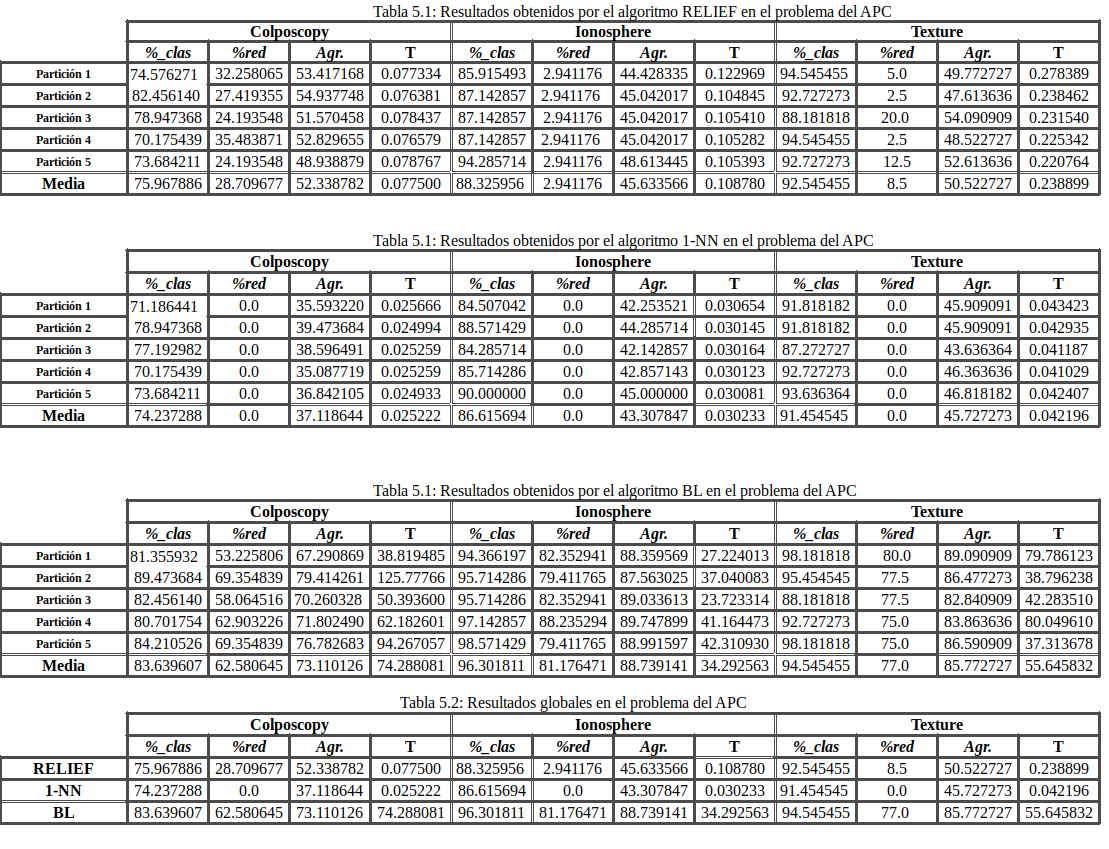
\includegraphics[width=1\linewidth]{screen3}
		\caption{}
		\label{fig:screen3}
	\end{figure}
	
	
	
	
	
	
	
	\subsubsection{Análisis de resultados}
	Los resultados obtenidos nos muestra que la búsqueda local es muy superior a las otras en cuanto a obtener mejores resultados y la que mayor tasa de reducción. Esto se debe a que es la que mas opciones comprueba y siempre se va quedando con la mejor. Con esto evita perder buenas soluciones. Ademas al solo aceptar la mutación cuando mejora tiende a mejorar rápido hasta que se cumplen las 20*n iteraciones sin mejora. Estas iteraciones sin mejora son siempre la causa de que termine el algoritmo sin llegar nunca a el máximo de vecinos generado. Suele generar unos 7000 vecinos la vez que mas y normalmente ronda entre 2000 y 4000 en textura por ejemplo.
	
	El siguiente que mejor resultados me suele dar es el RELIEF aunque el 1-nn no se diferencia tanto de el. Esto se trata a que el RELIEF si utiliza los datos de entrenamiento para intentar mejorar mediante la ponderación de los pesos. El 1-nn depende de lo parecidos que sean las particiones de entrenamiento y test puesto que no obtienen ningún tipo de mejora para aproximar sus datos a los de entrenamiento.
	
	Algo curioso es que en los ficheros de IONOSPHERE RELIEF siempre me reduce el mismo numero de pesos. Imagino que podrá ser por pesos que son muy parecidos para todos los elementos de la muestra. Y por eso los tiende a reducir al no ser significativos.
	
	El mejor conjunto de datos para el ajuste es textura. Llegando a obtener mas de 90\% de media para todos los datos. El mas difícil de clasificar correctamente es el colposcopy. Aunque en la función de evaluación mejora mucho colopscopy porque suele ser tener una buena tasa de reducción. Y al darle la misma importancia a la clasificación y la reducido eso hace que se la que mejor función objetivo tenga. Esto no se cumple por ejemplo en el 1-nn al no tener reducción es la que peor función objetivo tiene
	
	En la búsqueda local me sorprende que se capaz de ajustar tanto teniendo tasa reducción tan altas. Entiendo que con eso evitara mucho ruido que dan los datos eliminados
	
	\subsubsection{Tiempo de ejecución}
	El tiempo de ejecución de menor a mayor como era obvio el que menos tarda es el 1-nn puesto que los otros dos utilizan a este para la clasificación. Es prácticamente instantáneo
	
	Lo sigue el RELIEF que si el anterior tarda como el doble triple que esta pero tampoco es un tiempo considerable.
	
	La búsqueda local es mucho mas lenta. Conseguí reducirla mucho al tener en cuenta que hay ocasiones en las que no hacia falta volver a valorar un peso porque no es posible que este mejore. Llegue a bajar de tardar unos 10 minutos de media partición a 1.25 minutos la que mas me puede tardar. También es verdad que depende de la semilla en algunas condiciones. Siendo los datos en lo que mas tarda los que mas numero de características por elemento tienen.
	
	

	\section{Bibliografía}
	No he usado nada fuera de las propias paginas de información de python o de las librerías utilizadas como podría ser la de numpy.

  
\end{document}